\chapter{El cambio global y la biosfera}\label{ch:b2:global-change}

Entre 1851 y 1858, Henry Thoreau recorrió los bosques y prados de los
alrededores de Concord, en Massachusetts, y anotó el día en que florecía
por primera vez cada una de unas quinientas plantas. Siglo y medio más
tarde, unos botánicos volvieron a los mismos lugares con sus cuadernos. El
arándano alto que Thoreau veía abrirse el 11 de mayo se abre hoy el 12 de
abril; el conjunto de la flora florece, por término medio, diez días antes
que en su época, al mismo ritmo que una primavera \qty{2.4}{\celsius} más
cálida; y una cuarta parte de sus especies ha desaparecido de Concord --- no
al azar, sino las que no podían ajustar su floración a la temperatura. Los
capítulos anteriores han dado la maquinaria: los ciclos del
\cref{ch:b2:biogeochemical-cycles}, la selección y la deriva del
\cref{ch:b2:population-genetics}, la competencia y la especiación
del \cref{ch:b2:speciation}, los \omterm{def:b2:living-soil:soil}{suelos} del \cref{ch:b2:living-soil}.
Este capítulo pone cifras a lo que les está ocurriendo a los seres vivos
mientras una sola especie cambia la química del aire y del mar: cuánto
calentamiento por tonelada de carbono, cuántos días de adelanto de la
primavera por grado, cuántos metros cuesta arriba, cuánto ácido en el mar,
cuántas especies perdidas por hectárea --- y lo que dicen las cifras sobre
el siglo que viene.

\section{El cambio físico}

\begin{proposition}[El calentamiento es proporcional a las emisiones acumuladas]\label{prop:b2:global-change:tcre}
\index{calentamiento global}\index{emisiones acumuladas}\index{presupuesto de carbono}\index{efecto invernadero}
El dióxido de carbono absorbe el infrarrojo que emite el \omterm{def:b2:living-soil:soil}{suelo} y devuelve
una parte; más \ensuremath{\mathrm{CO_2}} significa una superficie más cálida, en
unos \qty{3}{\celsius} por cada duplicación una vez que los océanos se han
puesto al día (la \emph{sensibilidad climática}). Como la respuesta de la
temperatura al \ensuremath{\mathrm{CO_2}} es logarítmica en la concentración, mientras
que la \omterm{prop:b2:biogeochemical-cycles:carbon}{fracción atmosférica} de las emisiones disminuye a medida que sube
la concentración, las dos curvaturas casi se compensan, y el calentamiento
medio global es, con buena aproximación, \emph{lineal en la cantidad
acumulada de carbono emitido}, sea cual sea el calendario:
\[
\Delta T \approx \lambda\,C_{\text{acum}}, \qquad \lambda \approx
\qty{1.65}{\celsius} \text{ por } \qty{1000}{GtC}
\]
(\qty{0.45}{\celsius} por \qty{1000}{Gt} de \ensuremath{\mathrm{CO_2}}). Unas
\qty{700}{GtC} emitidas desde 1850 han calentado el planeta
\qty{1.2}{\celsius} --- y la relación asigna a cada objetivo un
presupuesto: \qty{1.5}{\celsius} permite unas \qty{900}{GtC} en total,
\qty{200}{GtC} más de lo ya emitido, veinte años al ritmo actual. El
calentamiento es desigual: el doble de la media sobre los continentes y el
triple en el Ártico; más de noche que de día; y viene acompañado del resto
--- lluvias más intensas y sequías más largas, un nivel del mar que sube
\qty{4}{mm} al año, un hielo estival una quinta parte más pequeño y un
océano que ha absorbido el \qty{90}{\%} del calor y una cuarta parte del
carbono.
\end{proposition}
\begin{proof}[Evidencia]
La proporcionalidad se encontró en modelos climáticos de todos los grados
de complejidad y la confirmó el registro observado: representar el
calentamiento desde 1850 frente a las \omterm{prop:b2:global-change:tcre}{emisiones acumuladas} da una línea
recta a lo largo de las décadas. El propio \omterm{prop:b2:global-change:tcre}{efecto invernadero} se mide desde
la órbita: los satélites ven el infrarrojo que emite la Tierra con las
bandas de absorción del \ensuremath{\mathrm{CO_2}}, del metano y del vapor de agua
recortadas, y el recorte se ha hecho más profundo entre 1970 y 2020
exactamente en la cantidad que predice el aumento de esos gases. Los
isótopos y el descenso del oxígeno del \cref{ch:b2:biogeochemical-cycles}
vinculan el \ensuremath{\mathrm{CO_2}} adicional con los combustibles fósiles.
\end{proof}
\begin{omfigure}
\begin{tikzpicture}
\begin{axis}[
  width=0.88\linewidth, height=5.6cm,
  axis x line=bottom, axis y line=left,
  xmin=1845, xmax=2030, ymin=-0.3, ymax=1.5,
  xlabel={década}, ylabel={calentamiento (\unit{\celsius}) desde 1850--1900},
  xlabel style={font=\small, at={(axis description cs:0.5,-0.13)}, anchor=north},
  ylabel style={font=\small},
  tick label style={font=\small}, xtick={1850,1900,1950,2000}, ytick={0,0.5,1,1.5},
  scaled x ticks=false, x tick label style={/pgf/number format/1000 sep=},
  clip=false,
]
\addplot[ybar, bar width=7pt, fill=omThm!50, draw=omThm] coordinates {
(1855,0.00) (1865,-0.04) (1875,0.02) (1885,-0.06) (1895,-0.02) (1905,-0.10) (1915,-0.06) (1925,0.05) (1935,0.15) (1945,0.25) (1955,0.15) (1965,0.15) (1975,0.18) (1985,0.40) (1995,0.55) (2005,0.78) (2015,1.02) (2023,1.28)};
\node[font=\scriptsize, anchor=west, align=left] at (axis cs:1850,1.2) {cada barra: la media de una década; la última, 2020--2024\\ \qty{700}{GtC} emitidas, $\qty{1.65}{\celsius}/\qty{1000}{GtC}$: \qty{1.2}{\celsius}};
\end{axis}
\end{tikzpicture}

{\small Temperatura media global de la superficie por décadas, respecto de
la segunda mitad del siglo XIX. Cada una de las cuatro últimas décadas ha
batido un récord, y la subida desde 1970 es de \qty{0.2}{\celsius} por
década.}
\end{omfigure}

\section{El calendario: la fenología}

\begin{theorem}[Los grados-día y el adelanto de la primavera]\label{thm:b2:global-change:phenology}
\index{fenología}\index{grados-día}\index{tiempo térmico}\index{desajuste fenológico}
Muchos acontecimientos de la vida de las plantas y de los ectotermos ---
la brotación, la floración, la eclosión de los huevos, la emergencia --- se
producen cuando el \emph{\omterm{thm:b2:global-change:phenology}{tiempo térmico}} acumulado desde una fecha de
partida, la suma de las temperaturas diarias por encima de una base $T_b$
(los \emph{grados-día}), alcanza un total fijo $K$. Si la temperatura
primaveral sube linealmente, $T(t) = T_b
+ b\,(t - t_0)$, a razón de $b$ grados por día desde el día $t_0$ en que
supera la base, el acontecimiento se produce en
\[
t^{*} = t_0 + \sqrt{2K/b},
\]
y un calentamiento uniforme $\Delta T$ adelanta el día en que se supera la
base en $\Delta T/b$, y el acontecimiento con él: con $b \approx
\qty{0.1}{\celsius}$ por día, \emph{unos diez días antes por
grado}. Las especies difieren en $T_b$, en $K$ y en si usan también la
duración del día, que el calentamiento no cambia --- de modo que los
miembros de una cadena trófica se adelantan a ritmos distintos y sus
calendarios se separan: un \emph{\omterm{thm:b2:global-change:phenology}{desajuste fenológico}} entre la oruga y
el ave que debe alimentar con ella a sus polluelos.
\end{theorem}
\begin{proof}
Grados-día desde $t_0$: $\int_{t_0}^{t}(T - T_b)\,\mathrm{d}t' =
b\,(t - t_0)^{2}/2$, igual a $K$ cuando $t - t_0 = \sqrt{2K/b}$.
Calentar en $\Delta T$ sustituye $T$ por $T + \Delta T$: la base se supera
$\Delta T/b$ días antes y la acumulación, idéntica a partir de ese día,
se completa $\Delta T/b$ días antes. (Si el calentamiento aumenta además
$b$, el intervalo $\sqrt{2K/b}$ también se acorta.) Una especie guiada por
la duración del día conserva su fecha; una guiada por los grados-día se
desplaza; la distancia entre ambas crece en $\Delta T/b$.
\end{proof}
\begin{proof}[Evidencia]
La flora de Concord de Thoreau y el registro de la familia Marsham de
veintisiete signos de la primavera en Norfolk, llevado entre 1736 y 1947,
muestran ambos un adelanto de la floración y de la foliación de
\qtyrange{3}{6}{d} por grado de calentamiento primaveral. La floración del
cerezo de Kioto, fechada en los diarios de la corte desde el siglo IX, se
mantuvo en torno a mediados de abril durante mil años y se ha desplazado a
principios de abril desde 1900, con las fechas más tempranas registradas en
la década de 2020. En los Países Bajos, las orugas del roble alcanzan hoy
su máximo dos semanas antes que en 1985; el carbonero común, guiado por el
mismo calor, ha seguido el ritmo, pero el papamoscas cerrojillo, que
programa su migración desde África según la duración del día, llega como
antes y encuentra el máximo ya pasado --- sus poblaciones han caído un
\qty{90}{\%} allí donde el desajuste es mayor (Both y sus colaboradores,
2006).
\end{proof}

\begin{omfigure}
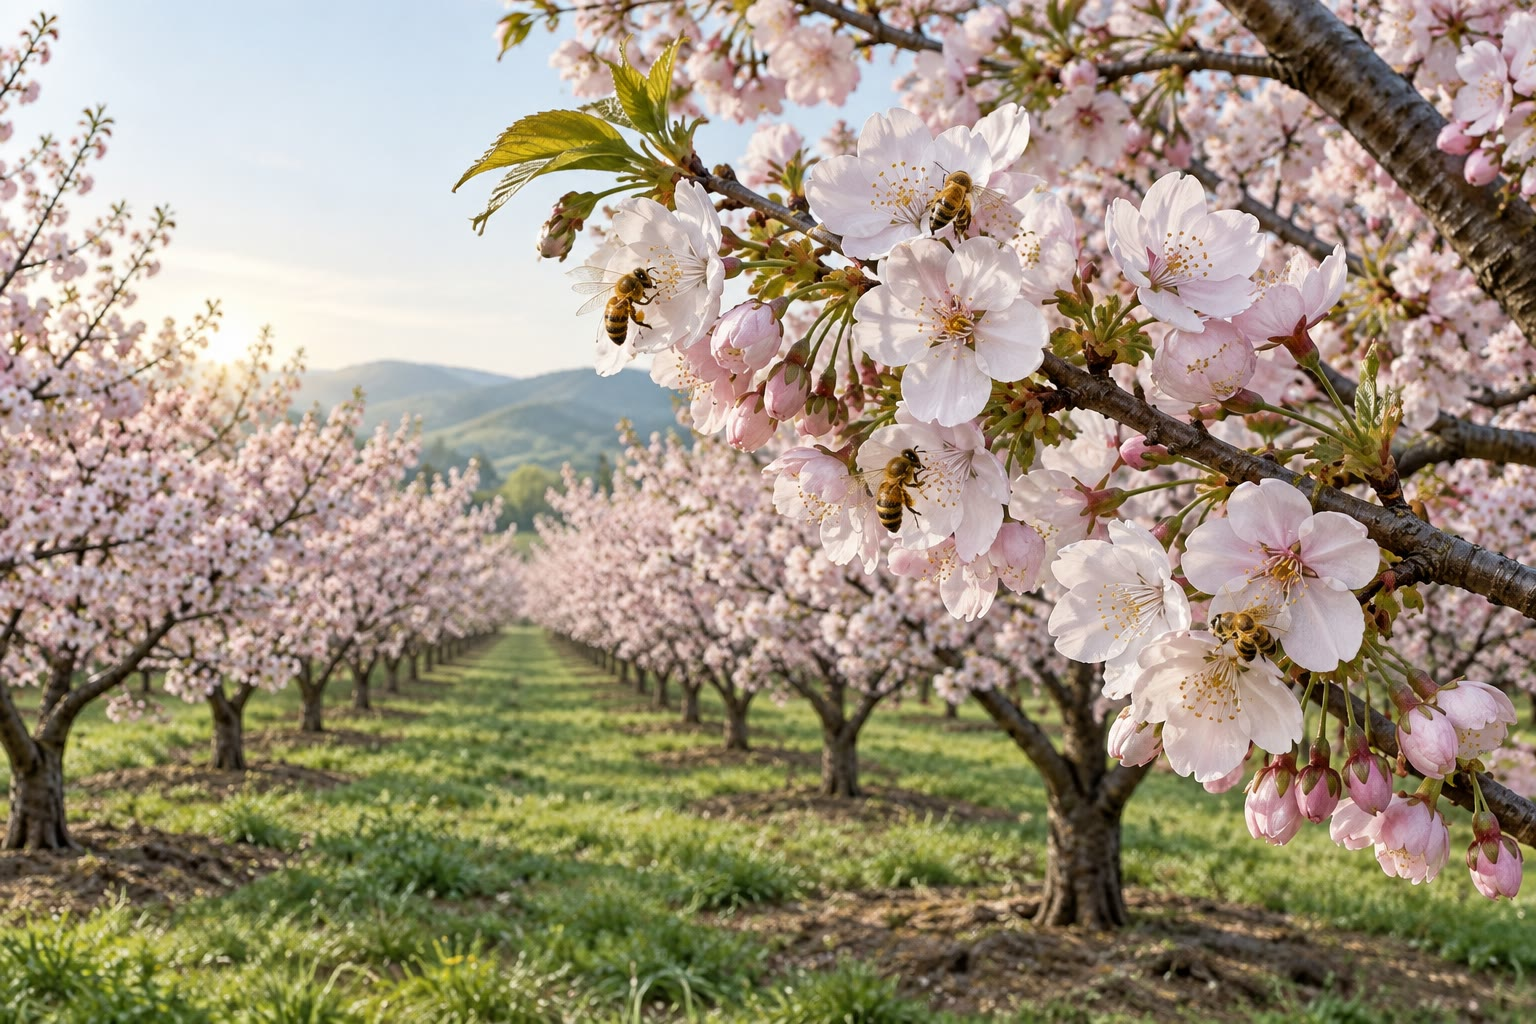
\includegraphics[width=0.62\linewidth]{images/book4/ai/b4-27-phenology-cherry.jpg}

{\small Un huerto de cerezos en \omterm{def:b2:angiosperm-reproduction:flower}{flor}. Los cerezos de Kioto, fechados en
diarios desde hace doce siglos, se abren hoy antes que en cualquier año
anterior a 1900 --- y las abejas que los polinizan tienen que volar ese
mismo día.}
\end{omfigure}

\begin{omfigure}
\begin{tikzpicture}
\begin{axis}[
  width=0.74\linewidth, height=5.4cm,
  axis x line=bottom, axis y line=left,
  xmin=0, xmax=100, ymin=0, ymax=14,
  xlabel={días desde el 1 de marzo}, ylabel={temperatura media diaria (\unit{\celsius})},
  xlabel style={font=\small, at={(axis description cs:0.5,-0.13)}, anchor=north},
  ylabel style={font=\small},
  tick label style={font=\small}, xtick={0,20,40,60,80,100},
  legend style={font=\scriptsize, at={(0.03,0.97)}, anchor=north west, draw=none},
  clip=false,
]
\addplot[very thick, omDef, domain=0:100, samples=2] {2 + 0.1*x};
\addlegendentry{primavera antes del calentamiento}
\addplot[very thick, omThm, domain=0:100, samples=2] {3 + 0.1*x};
\addlegendentry{primavera \qty{1}{\celsius} más cálida}
\draw[dashed, gray] (axis cs:0,5) -- (axis cs:100,5); \node[font=\scriptsize, anchor=south east] at (axis cs:100,5) {temperatura base $T_b = \qty{5}{\celsius}$};
\fill[omDef, opacity=0.15] (axis cs:30,5) -- (axis cs:93,5) -- (axis cs:93,11.3) -- cycle;
\fill[omThm, opacity=0.15] (axis cs:20,5) -- (axis cs:83,5) -- (axis cs:83,11.3) -- cycle;
\draw[<->, thick] (axis cs:83,1.6) -- (axis cs:93,1.6); \node[font=\scriptsize, anchor=south] at (axis cs:88,1.8) {10 días};
\draw[dotted] (axis cs:93,0) -- (axis cs:93,5); \draw[dotted] (axis cs:83,0) -- (axis cs:83,5);
\node[font=\scriptsize, anchor=south, align=center] at (axis cs:62,11.4) {$K = 200$ grados-día\\ (áreas sombreadas)};
\end{axis}
\end{tikzpicture}

{\small Grados-día. El acontecimiento se produce cuando el área sombreada
entre la recta de temperatura y la base alcanza $K$; una primavera un grado
más cálida supera la base diez días antes y completa la suma diez días
antes.}
\end{omfigure}

\section{El mapa: los desplazamientos de las áreas de distribución}

\begin{proposition}[Las isotermas se desplazan, y las especies las siguen]\label{prop:b2:global-change:range}
\index{desplazamiento del área de distribución}\index{velocidad climática}\index{gradiente térmico vertical}
La temperatura baja unos \qty{6.5}{\celsius} por kilómetro de altitud y
unos \qty{0.65}{\celsius} por cada cien kilómetros de latitud en la zona
templada; un calentamiento de \qty{1}{\celsius} desplaza, por tanto, cada
isoterma unos \qty{150}{m} cuesta arriba y \qty{150}{km} hacia el polo.
Las especies cuyos límites fija la temperatura se desplazan con su
isoterma si pueden: la media de cientos de especies estudiadas se ha
desplazado \qty{11}{m} cuesta arriba y \qty{17}{km} hacia el polo por
década desde 1970, a la velocidad de las isotermas, y las más rápidas ---
móviles, generalistas, de vida corta --- las adelantan, mientras que los
árboles, cuyas \omterm{def:b2:angiosperm-reproduction:seed}{semillas} viajan unos metros al año, y las especies que ya
están en la cima o en el polo no pueden seguirlas: la cima de una montaña
no tiene adónde ir, y cada grado de calentamiento elimina los
\qty{150}{m} superiores de cada área de distribución. Las especies
marinas, sin barreras y con límites térmicos más estrictos, se desplazan
más deprisa, decenas de kilómetros por década; el bacalao, la caballa y,
con ellos, las pesquerías se han desplazado hacia el norte a través de
mares enteros. El borde superior de un área de distribución avanza, el
borde inferior retrocede a medida que se calienta y que llegan nuevos
competidores desde abajo, y la comunidad de cada lugar se recompone con
especies que nunca se habían encontrado.
\end{proposition}
\begin{proof}[Evidencia]
Parmesan (1996) volvió a muestrear la mariposa damero de Edith
en toda su área del oeste de Norteamérica: las poblaciones del borde sur y
de baja altitud se habían extinguido, las del borde norte y de gran
altitud prosperaban, y el área entera se había desplazado
\qty{92}{km} hacia el norte y \qty{124}{m} hacia arriba --- la primera
especie de la que se demostró que había seguido las isotermas. Lenoir y
sus colaboradores (2008) compararon inventarios de plantas forestales de
1905--1985 con los de 1986--2005 en las montañas francesas: la altitud
óptima de 171 especies había subido \qty{29}{m} por década. Chen y sus
colaboradores (2011), sobre dos mil especies, hallaron desplazamientos de
dos a tres veces más rápidos que las estimaciones anteriores, y
proporcionales al calentamiento local.
\end{proof}

\begin{omfigure}
\begin{tikzpicture}[every node/.style={font=\scriptsize}, >=stealth]
  \fill[gray!25] (0,0) -- (3.5,4.2) -- (7,0) -- cycle;
  \draw[thick] (0,0) -- (3.5,4.2) -- (7,0);
  \foreach \y/\lab in {1.0/{\qty{12}{\celsius}}, 2.2/{\qty{8}{\celsius}}, 3.4/{\qty{4}{\celsius}}} { \draw[omDef, thick] ({\y/1.2},\y) -- ({7-\y/1.2},\y) node[right] {\lab}; }
  \foreach \y in {1.15,2.35,3.55} { \draw[omThm, thick, dashed] ({\y/1.2},\y) -- ({7-\y/1.2},\y); }
  \node[omThm, anchor=west, align=left] at (7.6,3.7) {discontinuas: las mismas isotermas\\ tras \qty{1}{\celsius} de calentamiento,\\ \qty{150}{m} más arriba};
  \fill[omProp!50] (0.83,1.0) -- (6.17,1.0) -- (5.17,2.2) -- (1.83,2.2) -- cycle;
  \node[align=center] at (3.5,1.6) {banda de una especie,\\ \qtyrange{1000}{1200}{m}};
  \draw[->, thick, omExo!80!black] (1.1,2.2) -- (1.1,2.9); \node[omExo!80!black, anchor=east, align=right] at (0.95,2.55) {la banda sube\\ y se estrecha};
  \node[anchor=north] at (3.5,-0.1) {una montaña: el área disminuye con la altitud, y la cima no tiene nada más alto};
\end{tikzpicture}

{\small Un \omterm{prop:b2:global-change:range}{desplazamiento del área de distribución} en una montaña. Cada
grado eleva las isotermas \qty{150}{m}; una especie sigue su banda hacia
arriba, hacia un área menor, y una banda que ya está en la cima se pierde.}
\end{omfigure}

\section{El mar: acidificación y calor}

\begin{theorem}[La acidificación]\label{thm:b2:global-change:acid}
\index{acidificación del océano}\index{sistema de los carbonatos}\index{estado de saturación}\index{blanqueamiento del coral}
El dióxido de carbono que se disuelve en el agua de mar forma ácido
carbónico, que se disocia: $\ensuremath{\mathrm{CO_2}} + \ensuremath{\mathrm{H_2O}} \rightleftharpoons \ensuremath{\mathrm{H^{+}}} +
\ensuremath{\mathrm{HCO_3^{-}}}$, con $[\ensuremath{\mathrm{H^{+}}}][\ensuremath{\mathrm{HCO_3^{-}}}]/[\ensuremath{\mathrm{CO_2}}] = K_1$.
El bicarbonato es la mayor reserva de carbono del océano y la alcalinidad
lo mantiene casi constante, de modo que
\[
[\ensuremath{\mathrm{H^{+}}}] \propto p_{\ensuremath{\mathrm{CO_2}}}, \qquad
\Delta\mathrm{pH} \approx -\log_{10}\frac{p_{\ensuremath{\mathrm{CO_2}}}}{p_0}
\]
--- o, más exactamente, $-0.9\log_{10}$ de ese cociente, porque el bicarbonato
sube un poco. De 280 a \qty{420}{ppm}, el pH superficial ha bajado
$0.15$, de $8.2$ a $8.05$: un aumento del \qty{40}{\%} de los iones
hidrógeno; a \qty{800}{ppm} bajaría $0.4$. Los iones hidrógeno adicionales
consumen carbonato, $\ensuremath{\mathrm{H^{+}}} + \ensuremath{\mathrm{CO_3^{2-}}} \to \ensuremath{\mathrm{HCO_3^{-}}}$, y
el \emph{\omterm{thm:b2:global-change:acid}{estado de saturación}} $\Omega$ del carbonato de calcio ---
el producto de las concentraciones de calcio y de carbonato dividido por
el producto de solubilidad --- baja en la misma proporción: las conchas y
los esqueletos de aragonito (corales, pterópodos) se forman con facilidad
con $\Omega > 3$, con dificultad cerca de 1, y se disuelven por debajo; la
superficie tropical, con $\Omega \approx 4$ antes de la industria y 3
hoy, llega a 2 con \qty{560}{ppm}, y las aguas superficiales polares,
frías y ricas en \ensuremath{\mathrm{CO_2}}, llegan antes a 1.
\end{theorem}
\begin{proof}
A partir del equilibrio, $[\ensuremath{\mathrm{H^{+}}}] = K_1[\ensuremath{\mathrm{CO_2}}]/[\ensuremath{\mathrm{HCO_3^{-}}}]$, y
$[\ensuremath{\mathrm{CO_2}}]$ es proporcional a $p_{\ensuremath{\mathrm{CO_2}}}$ según la ley de Henry;
con $[\ensuremath{\mathrm{HCO_3^{-}}}]$ constante, $[\ensuremath{\mathrm{H^{+}}}]$ es proporcional a
$p_{\ensuremath{\mathrm{CO_2}}}$ y $\mathrm{pH} = -\log_{10}[\ensuremath{\mathrm{H^{+}}}]$ varía en
$-\log_{10}$ del cociente. El segundo equilibrio, $[\ensuremath{\mathrm{H^{+}}}][\ensuremath{\mathrm{CO_3^{2-}}}]/[\ensuremath{\mathrm{HCO_3^{-}}}]
= K_2$, da $[\ensuremath{\mathrm{CO_3^{2-}}}] \propto 1/[\ensuremath{\mathrm{H^{+}}}] \propto
1/p_{\ensuremath{\mathrm{CO_2}}}$, de modo que $\Omega$ baja cuando sube $p_{\ensuremath{\mathrm{CO_2}}}$, y
el aumento del \qty{40}{\%} de $[\ensuremath{\mathrm{H^{+}}}]$ es una bajada del \qty{30}{\%}
del carbonato. (La química completa, con la variación del bicarbonato y
las actividades de los iones, da el factor $0.9$ y las cifras
observadas; la trata el volumen del tercer año.)
\end{proof}
\begin{proof}[Evidencia]
La estación oceánica situada al norte de Hawái mide cada mes el pH
superficial desde 1988: baja $0.0018$ al año, al mismo ritmo que el
\ensuremath{\mathrm{CO_2}} del Mauna Loa, que tiene encima, como exige la química.
Los pterópodos --- los caracoles del mar, alimento de salmones y ballenas
--- recogidos frente a la costa del Pacífico muestran sus conchas de
aragonito picadas y en disolución allí donde los afloramientos suben a la
superficie agua con $\Omega <
1$. El \omterm{thm:b2:global-change:acid}{blanqueamiento del coral} se debe al calor, no al ácido: cuando el
agua se mantiene \qty{1}{\celsius} por encima del máximo estival durante
unas semanas, el coral expulsa sus algas simbióticas y muere de hambre; la
Gran Barrera de Coral se blanqueó en 1998, 2002, 2016, 2017, 2020, 2022 y
2024, y ha perdido la mitad de su cobertura de coral desde 1995.
\end{proof}
\begin{omfigure}
\begin{tikzpicture}
\begin{axis}[
  width=0.68\linewidth, height=5.4cm,
  axis x line=bottom, axis y line=left,
  xmin=250, xmax=1000, ymin=7.6, ymax=8.3,
  xlabel={\ensuremath{\mathrm{CO_2}} atmosférico (ppm)}, ylabel={pH superficial},
  xlabel style={font=\small, at={(axis description cs:0.5,-0.13)}, anchor=north},
  ylabel style={font=\small},
  tick label style={font=\small}, xtick={280,420,560,800,1000}, ytick={7.6,7.8,8.0,8.2},
  clip=false,
]
\addplot[very thick, omDef, domain=250:1000, samples=60] {8.2 - 0.9*log10(x/280)};
\fill[omDef] (axis cs:280,8.2) circle (2pt); \node[font=\scriptsize, anchor=south west] at (axis cs:285,8.2) {1750};
\fill[omThm] (axis cs:420,8.04) circle (2pt); \node[font=\scriptsize, anchor=south west] at (axis cs:425,8.04) {2020s: $-0.15$, $+\qty{40}{\%}$ \ensuremath{\mathrm{H^{+}}}};
\fill[omThm] (axis cs:800,7.79) circle (2pt); \node[font=\scriptsize, anchor=south west] at (axis cs:805,7.79) {2100 con emisiones altas};
\node[font=\scriptsize, anchor=north east, align=right] at (axis cs:1000,8.28) {$\Omega_{\text{aragonito}}$, trópicos:\\ 4 en 1750, 3 hoy, 2 con \qty{560}{ppm}};
\end{axis}
\end{tikzpicture}

{\small pH del océano superficial frente al dióxido de carbono
atmosférico,
$\mathrm{pH} = 8.2 - 0.9\log_{10}(p/280)$. La escala es logarítmica: cada
décima de unidad supone una cuarta parte más de iones hidrógeno.}
\end{omfigure}

\begin{omfigure}
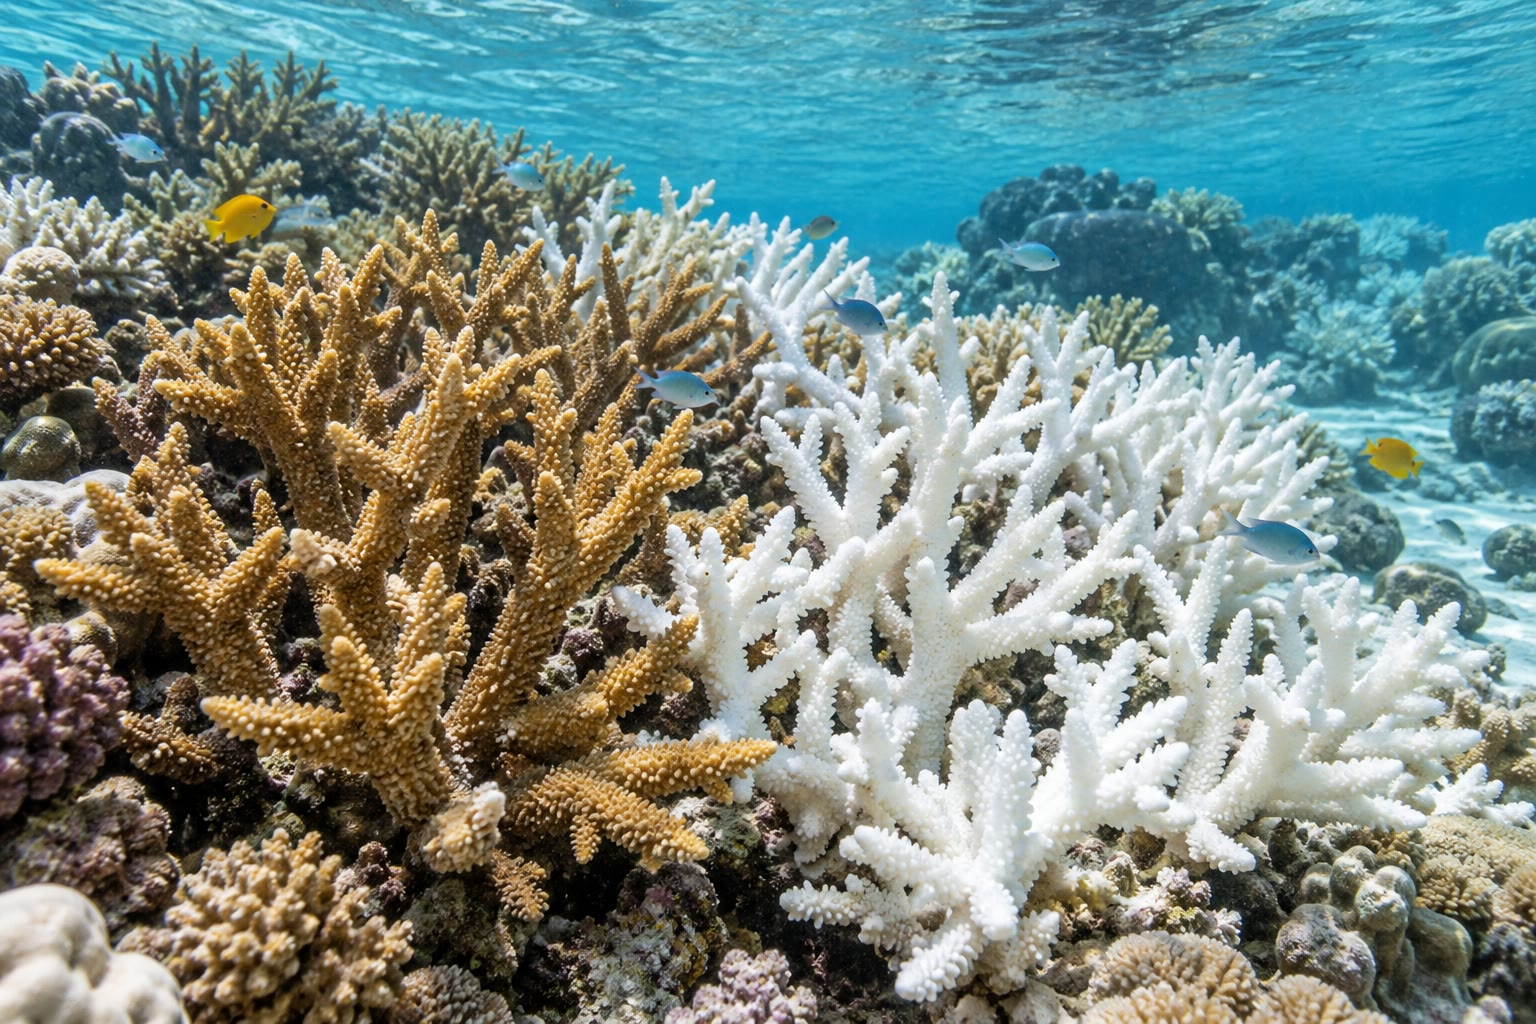
\includegraphics[width=0.44\linewidth]{images/book4/ai/b4-27-coral-bleaching.jpg}\hspace{0.04\linewidth}
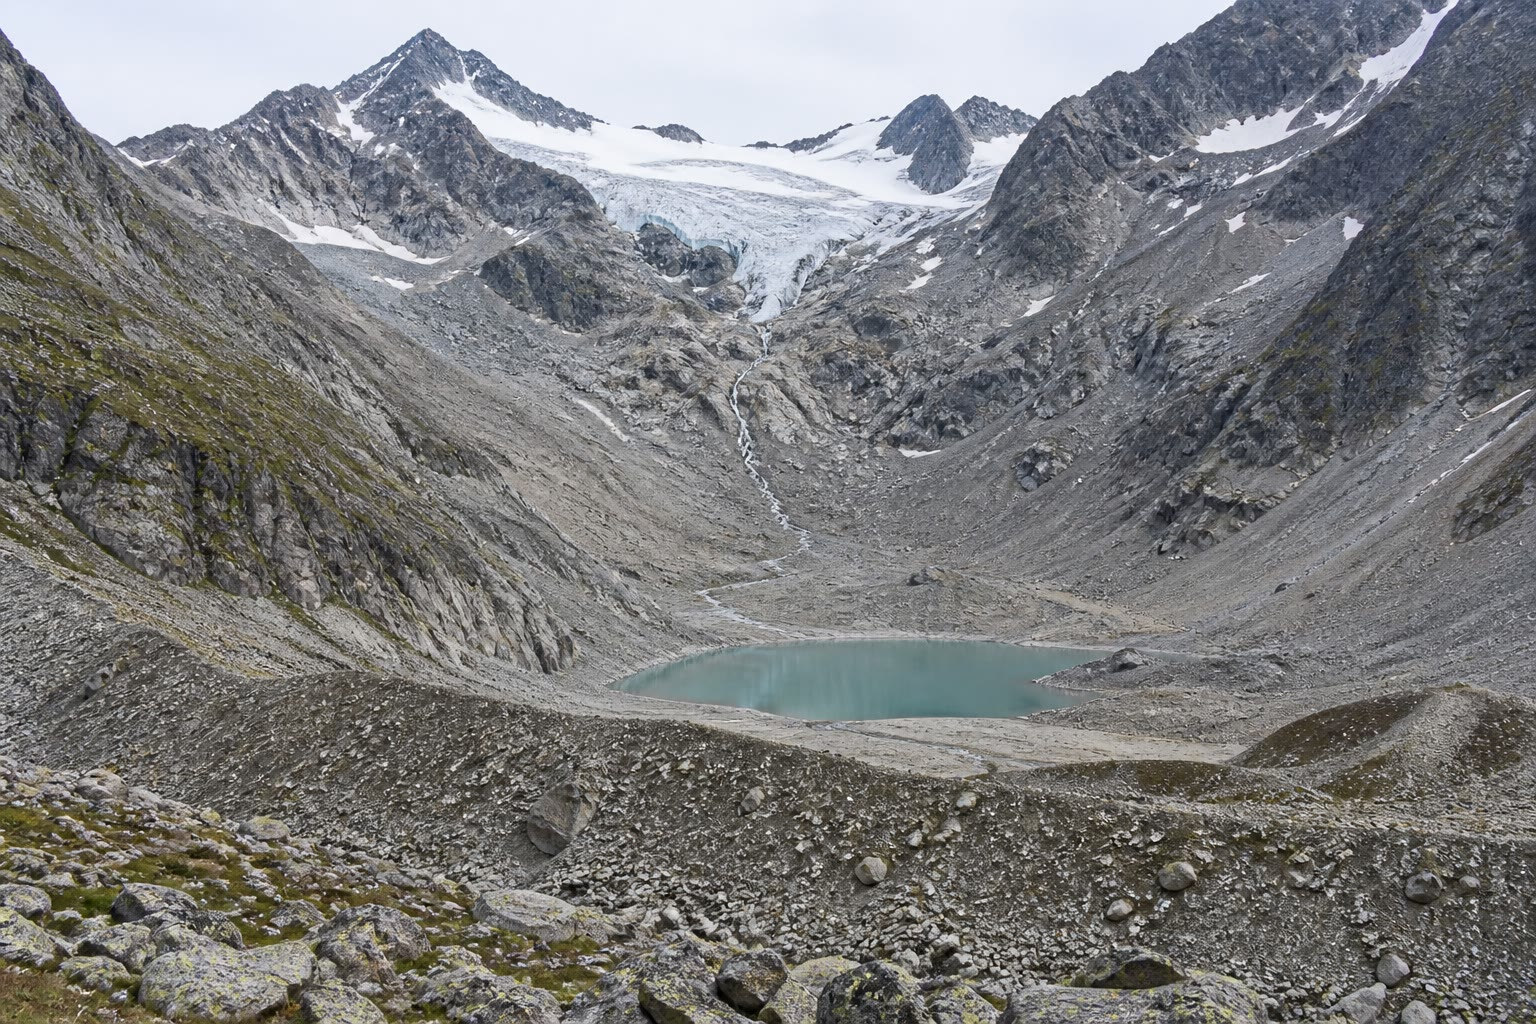
\includegraphics[width=0.44\linewidth]{images/book4/ai/b4-27-glacier-retreat.jpg}

{\small Dos termómetros. Izquierda: un arrecife blanqueado, con el
esqueleto blanco del coral visible a través de un tejido que ha perdido
sus algas. Derecha: un glaciar de valle que ha retrocedido valle arriba,
dejando roca desnuda donde hace un siglo había hielo.}
\end{omfigure}

\section{El balance: la extinción y su estimación}

\begin{theorem}[La relación especies--área y el coste de la pérdida de hábitat]\label{thm:b2:global-change:sar}
\index{relación especies--área}\index{tasa de extinción}\index{pérdida de hábitat}\index{deuda de extinción}
El número de especies que se encuentran en un área $A$ crece como una
potencia del área, $S = cA^{z}$, con $z \approx 0.25$ para las islas y los
fragmentos de hábitat (duplicar el área añade una quinta parte más de
especies; un área cien veces mayor, el triple de especies). Si un hábitat
se reduce a una fracción $1 - h$ de su extensión, el número de especies
que puede albergar a la larga baja a $(1 - h)^{z}$ del original: perder
la mitad del hábitat cuesta el \qty{16}{\%} de sus especies; el
\qty{90}{\%}, el \qty{44}{\%}; y el \qty{99}{\%}, el
\qty{68}{\%}. La pérdida no es inmediata --- los supervivientes del
fragmento persisten durante un tiempo, una \emph{\omterm{thm:b2:global-change:sar}{deuda de extinción}} que se
paga a lo largo de décadas a medida que las poblaciones pequeñas sucumben a
la deriva y a la endogamia del
\cref{ch:b2:population-genetics} ---, y es la base de la estimación según
la cual la tasa actual de extinción es de cien a mil veces la tasa de fondo
del registro fósil: alrededor de una especie de cada millón por año, frente
a las varias miles por año, de unos diez millones, que se pierden
actualmente.
\end{theorem}
\begin{proof}
$S'/S = (A'/A)^{z} = (1 - h)^{z}$; con $z = 0.25$, $0.5^{0.25} =
0.84$, $0.1^{0.25} = 0.56$, $0.01^{0.25} = 0.32$. La relación en sí es
empírica; su exponente refleja el equilibrio, en las islas, entre la
inmigración de especies nuevas (que disminuye a medida que la isla se
llena) y la extinción de las residentes (que aumenta a medida que sus
poblaciones se reducen con el área), el equilibrio de la teoría de
MacArthur y Wilson.
\end{proof}
\begin{proof}[Evidencia]
Las islas del grupo del Krakatoa, esterilizadas por la erupción de 1883,
fueron recolonizadas por plantas, aves e insectos en una sucesión que
alcanzó, en cincuenta años, el número de especies predicho a partir de sus
áreas; los islotes de manglar que Simberloff y Wilson fumigaron en Florida
en 1966 recuperaron su número original de especies, con especies
distintas, en un año. La mata atlántica de Brasil, reducida al
\qty{10}{\%} de su extensión, ha perdido o casi perdido la fracción de sus
especies de aves que predice la relación; y en todos los grupos evaluados
por la Unión Mundial para la Naturaleza, entre una cuarta y una tercera
parte de las especies están amenazadas --- aves, el
\qty{13}{\%}; mamíferos, el \qty{27}{\%}; anfibios, el \qty{41}{\%};
corales, el
\qty{44}{\%} ---, con la \omterm{thm:b2:global-change:sar}{pérdida de hábitat} como primera causa, y la caza,
las \omterm{prop:b2:global-change:invasion}{especies invasoras}, la contaminación y, cada vez más, el clima como las
demás.
\end{proof}
\begin{omfigure}
\begin{tikzpicture}
\begin{loglogaxis}[
  width=0.68\linewidth, height=5.4cm,
  axis x line=bottom, axis y line=left,
  xmin=1, xmax=100000, ymin=5, ymax=200,
  xlabel={área de la isla (\unit{km^2})}, ylabel={especies de aves terrestres},
  xlabel style={font=\small, at={(axis description cs:0.5,-0.13)}, anchor=north},
  ylabel style={font=\small},
  tick label style={font=\small},
  clip=false,
]
\addplot[only marks, mark=*, mark size=2pt, omDef] coordinates {(1.5,9) (8,14) (35,22) (150,32) (400,37) (1200,52) (4000,70) (13000,92) (35000,125) (85000,160)};
\addplot[very thick, omThm, domain=1:100000, samples=2] {9*x^0.25};
\node[font=\scriptsize, omThm, anchor=north west, align=left] at (axis cs:2,120) {$S = 9A^{0.25}$: un área cien\\ veces mayor, el triple\\ de especies};
\end{loglogaxis}
\end{tikzpicture}

{\small La \omterm{thm:b2:global-change:sar}{relación especies--área}, aquí para las aves terrestres de las
islas de un archipiélago: una recta de pendiente $z = 0.25$ en ejes
logarítmicos. Si se reduce un hábitat a una décima parte, conservará a la
larga poco más de la mitad de sus especies.}
\end{omfigure}

\begin{proposition}[Invasiones, servicios y lo que puede hacerse]\label{prop:b2:global-change:invasion}
\index{especie invasora}\index{servicios ecosistémicos}\index{mitigación}\index{emisiones netas nulas}
Los barcos, los aviones y el comercio han hecho pasar a miles de especies
más allá de las barreras que las mantenían separadas; la mayoría no llega
a establecerse, pero las pocas que lo logran --- el conejo en Australia, el
mejillón cebra en los Grandes Lagos, la culebra arborícola marrón que dejó
Guam sin aves, el hongo quitridio que ha llevado a la extinción a noventa
especies de anfibios --- se extienden como un frente que avanza a
velocidad constante, $c =
2\sqrt{rD}$ para una población que crece a una tasa $r$ y se dispersa con
un coeficiente de difusión $D$ (la rata almizclera de Skellam, liberada
cerca de Praga en 1905, se extendió por Europa a \qty{11}{km} al año, con
el radio de su área creciendo en línea recta con el tiempo). Frente a todo
esto está lo que la biosfera hace por su única especie problemática: la
\omterm{def:b2:angiosperm-reproduction:pollination}{polinización} de tres cuartas partes de los cultivos, la depuración del
agua, el control de las inundaciones, la \omterm{prop:b2:biogeochemical-cycles:nitrogen}{fijación del nitrógeno} y la
formación del \omterm{def:b2:living-soil:soil}{suelo}, las pesquerías, el carbono almacenado en los bosques
y los \omterm{def:b2:living-soil:soil}{suelos} --- los \emph{\omterm{prop:b2:global-change:invasion}{servicios ecosistémicos}}, valorados, allí donde
puede ponérseles precio, en más que el producto económico mundial. Lo que
puede hacerse se deduce de las cifras. El calentamiento se detiene cuando
se detienen las emisiones netas, y no antes: los \omterm{thm:b2:biogeochemical-cycles:box}{modelos de caja} del
\cref{ch:b2:biogeochemical-cycles} no admiten otra lectura de las
\emph{\omterm{prop:b2:global-change:invasion}{emisiones netas nulas}}. La tierra puede ayudar dentro de unos
límites --- una gigatonelada de carbono al año procedente de la
reforestación y los \omterm{def:b2:living-soil:soil}{suelos} durante unas décadas, frente a diez de los
combustibles fósiles ---, y se puede ayudar a las especies a desplazarse,
o mantenerlas en reservas lo bastante grandes y conectadas para que la
\omterm{thm:b2:global-change:sar}{relación especies--área} y la deriva de las poblaciones pequeñas no acaben
con ellas. Las herramientas son las de este libro: la \omterm{def:b2:population-genetics:frequencies}{genética de
poblaciones} de la reserva, la competencia del invasor, la fenología del
cultivo, el balance del \omterm{def:b2:living-soil:soil}{suelo}.
\end{proposition}

\begin{example}[Tres futuros]\label{ex:b2:global-change:scenarios}
Unas emisiones mantenidas en \qty{10}{GtC} al año hasta 2100 añaden
\qty{800}{GtC} a las \qty{700}{} ya emitidas: $1.65\times 1.5 =
\qty{2.5}{\celsius}$ a finales de siglo, y sigue subiendo. Unas emisiones
que bajan hasta cero en 2070 añaden unas \qty{250}{GtC}: \qty{1.6}{\celsius},
y después se estabiliza. Duplicar primero las emisiones, como hicieron las
primeras décadas del siglo, da \qty{4}{\celsius} o más. Las áreas de
distribución de la zona templada se desplazan \qty{200}{km} más allá de las
actuales en el primer caso y \qty{60}{km} en el segundo; la primavera
llega veinticinco días antes, o seis; el pH superficial llega a $7.8$, o se
mantiene cerca de
$8.0$; y las estimaciones de extinción, que dependen a la vez del hábitat y
del calentamiento, van de una décima a una tercera parte de las especies.
La diferencia entre los futuros es el área acumulada bajo una curva, que es
la suma de decisiones que todavía no se han tomado.
\end{example}

\section{Ejercicios}

\begin{exercise}[$\star$]\label{exo:b2:global-change:1}
Enúnciese la relación entre el calentamiento y las \omterm{prop:b2:global-change:tcre}{emisiones acumuladas}, y
calcúlese el calentamiento para unas \omterm{prop:b2:global-change:tcre}{emisiones acumuladas} de 700, 1000 y
\qty{2000}{GtC}.
\end{exercise}

\begin{exercise}[$\star$]\label{exo:b2:global-change:2}
Defínanse grados-día y \omterm{thm:b2:global-change:phenology}{desajuste fenológico}, con el papamoscas como
ejemplo.
\end{exercise}

\begin{exercise}[$\star$]\label{exo:b2:global-change:3}
¿Cuánto se desplazan las isotermas cuesta arriba y hacia el polo por grado
de calentamiento, y por qué no puede seguirlas una especie de la cima de
una montaña?
\end{exercise}

\begin{exercise}[$\star$]\label{exo:b2:global-change:4}
Explíquese en tres frases por qué añadir \ensuremath{\mathrm{CO_2}} al mar baja su
pH y su carbonato, y qué organismos resultan perjudicados.
\end{exercise}

\begin{exercise}[$\star\star$]\label{exo:b2:global-change:5}
Calcúlese el \omterm{prop:b2:global-change:tcre}{presupuesto de carbono} restante para \qty{1.5}{\celsius} y
para \qty{2}{\celsius} con $\lambda = \qty{1.65}{\celsius}$ por
\qty{1000}{GtC} y \qty{700}{GtC} ya emitidas; conviértanse ambos en años
a \qty{10}{GtC/yr}.
\end{exercise}

\begin{exercise}[$\star\star$]\label{exo:b2:global-change:6}
La primavera se calienta a $b = \qty{0.12}{\celsius}$ por día desde una
base de \qty{5}{\celsius}; una polilla necesita $K = 150$ grados-día.
Calcúlense los días que van desde que se supera la base hasta la
emergencia, y el adelanto para un calentamiento de \qty{1.5}{\celsius}.
\end{exercise}

\begin{exercise}[$\star\star$]\label{exo:b2:global-change:7}
El área de distribución de una planta abarca \qtyrange{800}{1400}{m} en
una montaña de \qty{1800}{m} de altura cuya área se reduce a la mitad cada
\qty{300}{m} de altitud. Tras \qty{3}{\celsius} de calentamiento, ¿dónde
está la banda y cuánta área ha perdido? ¿Y tras \qty{5}{\celsius}?
\end{exercise}

\begin{exercise}[$\star\star$]\label{exo:b2:global-change:8}
Calcúlense el pH superficial y el aumento de la concentración de iones
hidrógeno con 560, 800 y \qty{1000}{ppm}, a partir de $\mathrm{pH} = 8.2 -
0.9\log_{10}(p/280)$.
\end{exercise}

\begin{exercise}[$\star\star$]\label{exo:b2:global-change:9}
Con $z = 0.25$, ¿qué fracción de las especies se pierde a la larga cuando
se destruye el \qty{70}{\%}, el \qty{95}{\%} y el \qty{99.9}{\%} de un
hábitat? ¿Por qué la pérdida inmediata es menor?
\end{exercise}

\begin{exercise}[$\star\star\star$]\label{exo:b2:global-change:10}
Un invasor crece a $r = 0.7$ por año y se dispersa con $D =
\qty{20}{km^2/yr}$. Calcúlense la velocidad de su frente y el tiempo que
tarda en atravesar un país de \qty{1000}{km} de ancho. ¿Qué reduce la
velocidad a la mitad: reducir $r$ a la mitad o reducir $D$ a la mitad?
\end{exercise}

\begin{exercise}[$\star\star\star$]\label{exo:b2:global-change:11}
La \omterm{thm:b2:global-change:sar}{tasa de extinción} de fondo es de 1 por millón de especies-año y hay 8
millones de especies. Calcúlense las extinciones esperadas por año y por
siglo con la tasa de fondo, y con 1000 veces la tasa de fondo. Compárese
con las diez mil extinciones documentadas del último siglo y coméntese la
discrepancia.
\end{exercise}

\begin{exercise}[$\star\star\star$]\label{exo:b2:global-change:12}
``El calentamiento se detiene cuando se detienen las emisiones netas.''
Justifíquese a partir del \omterm{thm:b2:biogeochemical-cycles:box}{modelo de caja} de la atmósfera y de la
proporcionalidad entre el calentamiento y las \omterm{prop:b2:global-change:tcre}{emisiones acumuladas}, e
indíquese qué le falta al argumento.
\end{exercise}

\section{Problema: la biosfera en 2100}

\begin{problem}[{Problema de fin de semana --- dos trayectorias de emisiones
llevadas hasta 2100: el calentamiento de cada una, la primavera que
produce, la distancia que recorren sus isotermas, el ácido que pone en el
mar y las especies que cuesta a un bosque, hasta llegar a los dos
calentamientos, los dos valores de pH y la fracción de especies
perdidas}]
\label{pb:b2:global-change:1}
Datos. $\lambda = \qty{1.65}{\celsius}$ por \qty{1000}{GtC};
\qty{700}{GtC} emitidas hasta 2020 (calentamiento de \qty{1.2}{\celsius}).
Trayectoria A: \qty{10}{GtC/yr} constantes hasta 2100. Trayectoria B:
bajada lineal hasta cero en 2070. La primavera se calienta a
$b = \qty{0.1}{\celsius}$ por día por encima de una base de
\qty{5}{\celsius}; un árbol necesita $K = 200$ grados-día para echar las
hojas, y un ave migratoria llega en una fecha fija, 20 días después de la
foliación del árbol en 2020. \omterm{prop:b2:global-change:range}{Gradiente térmico vertical},
\qty{6.5}{\celsius/km}; gradiente latitudinal, \qty{0.65}{\celsius} por
\qty{100}{km}. Océano: $\mathrm{pH} = 8.2 - 0.9\log_{10}(p/280)$;
\ensuremath{\mathrm{CO_2}} en 2100: \qty{600}{ppm} en la trayectoria A, \qty{420}{ppm}
en la trayectoria B. Una región forestal de \qty{e5}{km^2} con 400
especies de árboles, $z = 0.25$, pierde por talas el \qty{60}{\%} de su
área hasta 2100 en la trayectoria A y el \qty{20}{\%} en la trayectoria B.

\medskip
\noindent\textbf{Parte I --- El calentamiento.}
\begin{enumerate}
  \item Calcúlense las \omterm{prop:b2:global-change:tcre}{emisiones acumuladas} en 2100 en cada trayectoria.
  \item Calcúlese el calentamiento en 2100 en cada trayectoria.
  \item Calcúlese el calentamiento en 2050 en cada una.
  \item ¿Cuál es la velocidad de calentamiento por década en la
        trayectoria A? Compárese con los \qty{0.2}{\celsius} por década
        observados.
  \item En la trayectoria B, ¿se detiene el calentamiento en 2070? ¿Por
        qué, según la proporcionalidad?
  \item ¿Qué emisión acumulada corresponde a \qty{2}{\celsius}, y en qué
        año la alcanza la trayectoria A?
\end{enumerate}

\medskip
\noindent\textbf{Parte II --- La primavera.}
\begin{enumerate}[resume]
  \item Calcúlense los días que van desde que se supera la base hasta la
        foliación en 2020.
  \item Calcúlese el adelanto de la foliación, respecto de 2020, en 2100
        en cada trayectoria (calentamiento respecto de 2020).
  \item La fecha de llegada del ave no cambia. Calcúlese el intervalo entre
        la foliación y la llegada en cada trayectoria en 2100.
  \item Las orugas que necesita el ave alcanzan su máximo 15 días después
        de la foliación y duran 10 días. ¿En qué trayectoria las encuentra
        todavía el ave?
  \item Supóngase en cambio que el ave se adelanta \qty{3}{d} por
        grado. Vuélvase a calcular el intervalo en la trayectoria A.
  \item Explíquese en una frase por qué lo que amenaza al ave es el
        desajuste, y no el calentamiento en sí.
\end{enumerate}

\medskip
\noindent\textbf{Parte III --- Las áreas de distribución.}
\begin{enumerate}[resume]
  \item Calcúlense el desplazamiento en altitud y en latitud de las
        isotermas en cada trayectoria, respecto de 2020.
  \item Una especie de árbol se dispersa \qty{100}{m} al año. ¿Puede
        seguir las isotermas hacia el polo en la trayectoria A? ¿Y en la B?
  \item Una especie ocupa \qtyrange{1500}{1800}{m} en una montaña de
        \qty{2000}{m}. En la trayectoria A, ¿dónde se sitúa su banda en
        2100, y qué ocurre?
  \item El área de la montaña se reduce a la mitad cada \qty{300}{m}.
        Calcúlese el factor de área que pierde esa especie en la
        trayectoria B.
  \item Un pez marino sigue las isotermas a \qty{30}{km} por década. ¿Es
        suficiente en la trayectoria A?
  \item Explíquese por qué el borde inferior de un área de distribución
        retrocede incluso donde la especie podría tolerar el calor.
\end{enumerate}

\medskip
\noindent\textbf{Parte IV --- El mar y el bosque.}
\begin{enumerate}[resume]
  \item Calcúlense el pH superficial en 2100 en cada trayectoria y el
        aumento de la concentración de iones hidrógeno desde 1750.
  \item El \omterm{thm:b2:global-change:acid}{estado de saturación} $\Omega$ de la superficie tropical era de
        4 en 1750 y baja como $[\ensuremath{\mathrm{H^{+}}}]^{-1}$. Calcúlese en 2100
        en cada trayectoria e indíquese lo que significa para el coral.
  \item Calcúlense el número de especies de árboles que puede albergar a la
        larga la región forestal en cada trayectoria y el número de
        especies perdidas.
  \item El calentamiento añade pérdidas: supóngase que cada grado por
        encima de 2020 elimina otro \qty{5}{\%} de las especies
        supervivientes. Vuélvanse a calcular las especies que quedan en
        cada trayectoria.
  \item Dese la fracción de las 400 especies perdida en cada trayectoria.
  \item ¿Cuál de las dos causas, la tala o el calentamiento, domina en cada
        trayectoria?
  \item Enúnciese el resultado: el calentamiento, el pH y la fracción de
        especies de árboles perdidas en 2100 en cada trayectoria.
\end{enumerate}
\end{problem}
